\documentclass[11pt,a4paper]{article}
\usepackage[utf8]{inputenc}
\usepackage[T1]{fontenc}
\usepackage[brazil]{babel}
\usepackage{amsmath,amssymb,bm}
\usepackage{graphicx,booktabs,float,geometry,hyperref}
\geometry{margin=2.2cm}
\providecommand{\versao}{sem versao}
\newcommand{\Pf}{P_f}
\title{Viga com campo aleatório em Mathematica:\\ Monte Carlo, FORM, SORM e amostragem por importância (ISMC)}
\author{Diogo Cecílio}
\date{19/11/2026 --- versão \versao}
\begin{document}
\maketitle
\begin{abstract}
Um exemplo pequeno, em Mathematica, para testar os métodos de confiabilidade do artigo da amostragem por importância
antes de usá-los no talude. Uma viga biapoiada 2D (MEF em estado plano de tensão) tem o módulo de elasticidade como um
campo lognormal discretizado pela KL de Nyström, e a falha é a flecha no meio do vão acima de um limite. Comparamos o
Monte Carlo direto, o FORM, o SORM e a amostragem por importância (ISMC) centrada no ponto de projeto. As perguntas são
quantos termos o campo precisa, quantos termos o FORM precisa para dar uma boa função de amostragem, e se o SORM melhora
essa função. Resposta curta: a ISMC não tem viés com qualquer centro; o centro do FORM com 8 a 20 termos, aplicado ao
campo completo, dá CoV de 5\,\% com $\approx 1200$ análises, contra 18\,666 do Monte Carlo direto (15$\times$); o SORM
corrige a $\Pf$ do FORM (de $-21$ para $-5\,\%$), mas como função de amostragem quase não ajuda (1 a 2\,\% menos
amostras) e o hessiano custa mais do que economiza.
\end{abstract}
\tableofcontents

\section{O código}
Os dois arquivos estão em \path{codigo/} (cópias de \path{~/Dropbox/UnsaturatedSoil/mathematica}):
\begin{itemize}
  \item \texttt{viga\_estudo\_M\_ISMC.txt}: o estudo em $M$ (seções 0 a 23): Nyström com até 500 modos, MC, FORM e ISMC
    para cada $M$, as fórmulas de viga (Timoshenko \& Goodier e Euler--Bernoulli) como centros baratos e a ISMC no campo de
    500 modos;
  \item \texttt{viga\_FORM5\_AI200.txt}: FORM com 5 termos e ISMC com 200 (seções 1 a 10), o pós-processamento (11), o
    ponto ótimo (12), o SORM (13), a ISMC com o SORM (14) e a verificação SORM $\times$ FORM (15).
\end{itemize}
Cada resultado caro (MC, FORM, ISMC, hessiano) fica num arquivo \texttt{.mx} na pasta do notebook e só roda uma vez.

\section{O problema}
\begin{itemize}
  \item \textbf{Viga:} $5 \times 1$ (espessura 1), biapoiada ($v = 0$ nas faces das pontas, $u = 0$ no canto), carga
    $q = 1$ para baixo na face de cima, $\nu = 0{,}3$. MEF do Mathematica (\texttt{NDSolve}, malha de ordem 2,
    \texttt{MaxCellMeasure} 0,05), estado plano de tensão.
  \item \textbf{Conferência determinística} ($E = 200\,000$): no meio do vão, o MEF dá $5{,}3258\times10^{-4}$, a
    solução 2D de Timoshenko \& Goodier $5{,}3281\times10^{-4}$ (0,04\,\%), Euler--Bernoulli $4{,}883\times10^{-4}$ e a viga
    de Timoshenko ($\kappa = 5/6$) $5{,}370\times10^{-4}$.
  \item \textbf{Campo:} $E(\bm x)$ lognormal, média 200\,000 e CoV 0,3; o gaussiano tem covariância exponencial
    $\exp(-|\Delta x|/1 - |\Delta y|/0{,}5)$. KL de Nyström na malha de ordem 1 com \texttt{MaxCellMeasure} 0,0025
    (2121 nós, pesos de área), $E$ interpolado nos nós do MEF pela fórmula de Nyström.
  \item \textbf{Falha:} flecha no meio do vão $\delta > \delta_{lim} = 0{,}00075$; $g(\bm\xi) = \delta_{lim} - \delta(\bm\xi)$.
\end{itemize}

\section{Os métodos}
\begin{itemize}
  \item \textbf{MC direto:} $\hat P_f = $ fração de falhas; CoV $= \sqrt{(1-P_f)/(N P_f)}$; para CoV de 5\,\%,
    $N = (1-P_f)/(0{,}05^2 P_f)$.
  \item \textbf{FORM:} HL-RF no espaço dos $\xi$ (já normais padrão), gradiente por diferenças centrais com $h = 0{,}1$
    (2M análises por iteração, em paralelo); $P_f = \Phi(-\beta)$.
  \item \textbf{ISMC:} $\bm\xi \sim h = N(\bm\mu, \Sigma)$, $\hat P_f = \frac1N\sum I_k w_k$, $w = \varphi/h$ exato. Com o
    centro do FORM de $m$ termos num campo de $M > m$ termos, $\bm\mu = (\bm\xi^*_m, 0, \ldots, 0)$: o peso continua
    exato e o estimador sem viés; o centro só muda a variância.
  \item \textbf{CoV verdadeiro sem MEF:} $\mathrm{Var}_h(Iw) = P_f\,E_\varphi[w \mid \text{falha}] - P_f^2$, com a média
    sobre as falhas do MC direto. Dá o $N$ da ISMC para CoV de 5\,\% de qualquer centro sem rodar o MEF.
  \item \textbf{SORM:} hessiano de $g$ por diferenças finitas no $\bm\xi^*$ ($h = 0{,}2$; $M(M-1) + 2M + 1$ análises);
    curvaturas $\kappa_i$ = autovalores do hessiano no plano tangente dividido por $|\nabla g|$; Breitung
    $P_f = \Phi(-\beta)\prod(1+\beta\kappa_i)^{-1/2}$ e Hohenbichler--Rackwitz com $\psi = \varphi(\beta)/\Phi(-\beta)$ no
    lugar de $\beta$.
  \item \textbf{ISMC com o SORM:} $h = N(\bm\xi^*, \Sigma)$, $\Sigma = \bm n\bm n^T + R^T(I + cK)^{-1}R$ nos $m$ primeiros
    modos ($c = \beta$ ou $\psi$) e a identidade nos outros.
\end{itemize}

\section{O truncamento e a ISMC em cada M}
\begin{table}[H]\centering\small
\resizebox{\ifdim\width>\textwidth\textwidth\else\width\fi}{!}{%
\begin{tabular}{rrrrrrrr}
\toprule
$M$ & variância & $P_f$ MC (20\,000) & $\beta$ FORM & $P_f$ FORM & $P_f$ ISMC (1000) & CoV ISMC & $z$ (vs MC do mesmo $M$) \\
\midrule
5 & 0,491 & 1,33\,\% & 2,277 & 1,14\,\% & 1,30\,\% & 5,2\,\% & $-0{,}32$ \\
10 & 0,631 & 1,70\,\% & 2,149 & 1,58\,\% & 1,94\,\% & 5,0\,\% & 1,82 \\
20 & 0,746 & 1,95\,\% & 2,130 & 1,66\,\% & 1,85\,\% & 5,2\,\% & $-0{,}70$ \\
40 & 0,833 & 2,10\,\% & 2,130 & 1,66\,\% & 2,08\,\% & 5,0\,\% & $-0{,}15$ \\
100 & 0,915 & 2,15\,\% & 2,120 & 1,70\,\% & 2,08\,\% & 4,8\,\% & $-0{,}51$ \\
200 & 0,958 & 2,14\,\% & 2,118 & 1,71\,\% & 2,21\,\% & 4,7\,\% & 0,47 \\
\bottomrule
\end{tabular}}
\caption{MC direto, FORM e ISMC no ponto de projeto do mesmo $M$. A $P_f$ se estabiliza a partir de $M \approx 40$
(83\,\% da variância). O FORM subestima ~20\,\%. A ISMC acerta em todos os $M$ ($|z| < 2$).}
\end{table}
\begin{figure}[H]\centering
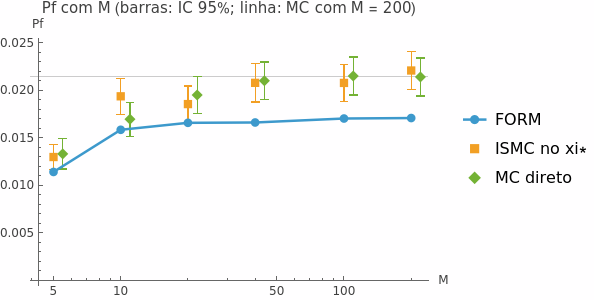
\includegraphics[width=0.48\textwidth]{figs/gPfM.png}\hfill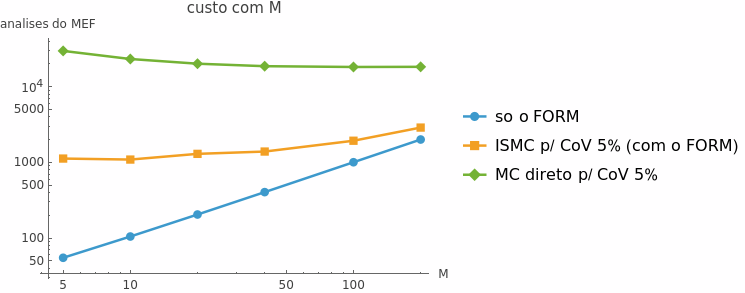
\includegraphics[width=0.48\textwidth]{figs/gCustoM.png}
\caption{$P_f$ com $M$ (barras: IC 95\,\%) e o custo para CoV de 5\,\%: o FORM por diferenças centrais custa $2M+1$ por
iteração, e o ganho da ISMC sobre o MC cai de 26$\times$ ($M = 5$) a 6$\times$ ($M = 200$).}
\end{figure}
\begin{figure}[H]\centering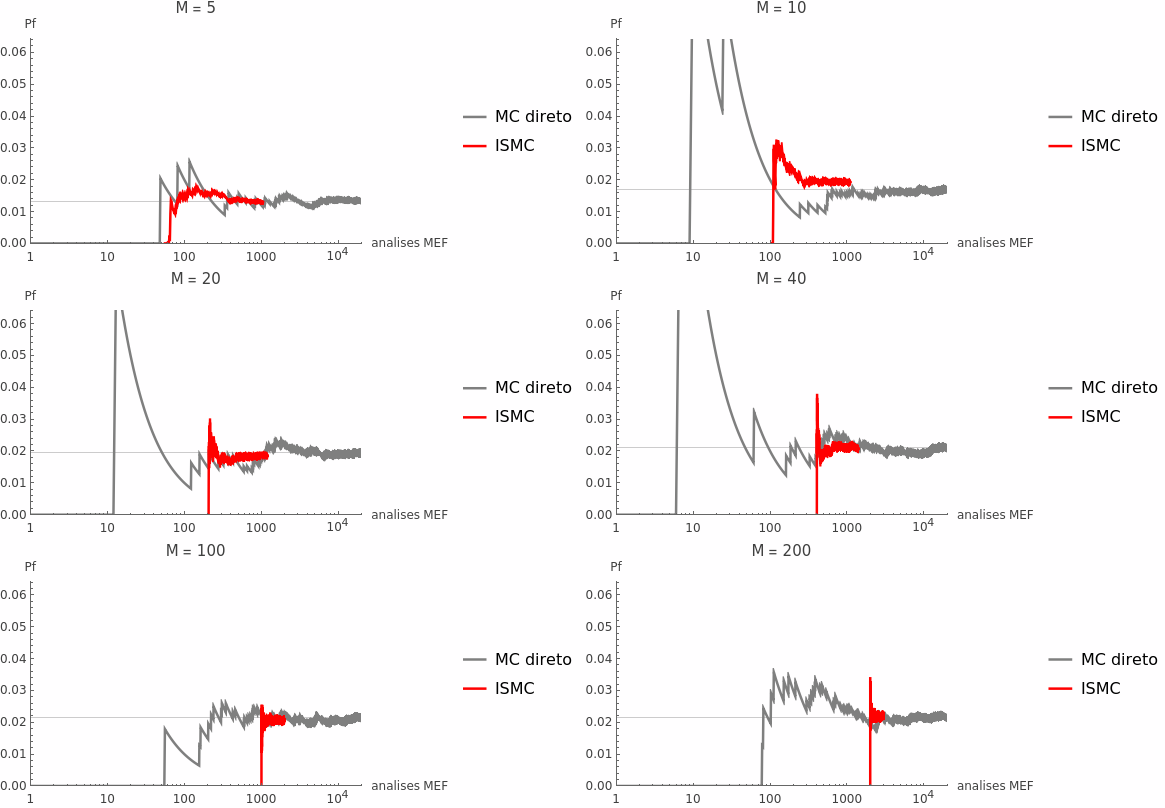
\includegraphics[width=0.85\textwidth]{figs/gConvM.png}
\caption{Convergência da $P_f$ da ISMC (vermelho, depois das análises do FORM) e do MC direto do mesmo $M$ (cinza).}
\end{figure}

\section{Centros baratos: fórmulas de viga no lugar do MEF}
A flecha de uma viga com $E(x,y)$ por trabalho virtual, com $EI(x)$ e $GA(x)$ integrados na altura (Simpson na grade de
Nyström): Euler--Bernoulli (só flexão) e Timoshenko \& Goodier (com o cortante, $\kappa = 0{,}912$, que reproduz a
solução 2D com $E$ constante). Cada avaliação leva 0,07\,ms. A correlação com o MEF nas 20\,000 amostras é 0,991
(TG) e 0,989 (EB); o EB subestima a flecha em 8,5\,\% e a sua $P_f$ em 4 a 5 vezes.
\begin{table}[H]\centering\small
\resizebox{\ifdim\width>\textwidth\textwidth\else\width\fi}{!}{%
\begin{tabular}{rlrrrrr}
\toprule
$M$ & centro & $\beta$ & $P_f$ ISMC & $z$ & análises p/ CoV 5\,\% & ganho vs MC \\
\midrule
20 & FORM-MEF & 2,13 & 1,85\,\% & $-0{,}70$ & 1297 & 15,5$\times$ \\
20 & FORM-TG & 2,12 & 1,88\,\% & $-0{,}47$ & 1096 & 18,4$\times$ \\
20 & FORM-EB & 2,64 & 2,19\,\% & 1,63 & 1067 & 18,9$\times$ \\
200 & FORM-MEF & 2,12 & 2,21\,\% & 0,47 & 2884 & 6,3$\times$ \\
200 & FORM-TG & 2,12 & 2,21\,\% & 0,50 & 949 & 19,3$\times$ \\
200 & FORM-EB & 2,64 & 2,03\,\% & $-0{,}69$ & 1293 & 14,2$\times$ \\
\bottomrule
\end{tabular}}
\caption{ISMC com o MEF centrada no ponto de projeto de cada FORM. Os FORM das fórmulas não gastam análises do MEF.}
\end{table}
\begin{figure}[H]\centering
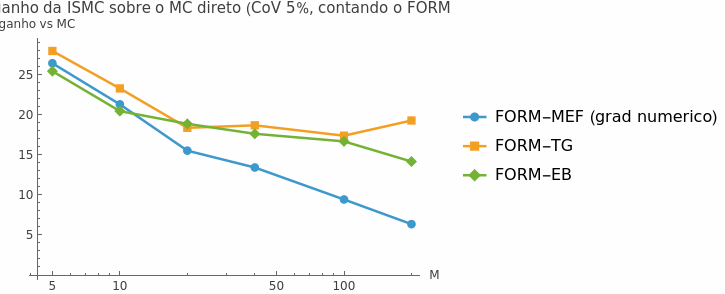
\includegraphics[width=0.48\textwidth]{figs/gGanhoCentros.png}\hfill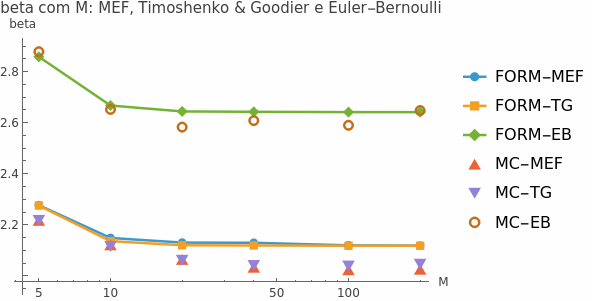
\includegraphics[width=0.48\textwidth]{figs/gBetaAnal.png}
\caption{Ganho da ISMC por centro e o $\beta$ com $M$ para o MEF, TG e EB.}
\end{figure}

\section{Centro de poucos termos no campo completo}
Com 500 modos (99\,\% da variância), o centro do FORM-MEF de 20 termos e 10 sementes de 1000 amostras: $P_f = 2{,}015\,\%$
(CoV 1,4\,\% nas 10 juntas) contra 1,895\,\% (CoV 5,1\,\%) do MC direto de 20\,000 com 500 modos ($z = 1{,}2$). O CoV
verdadeiro de uma ISMC de 1000 é 5,35\,\%, o estimado 5,10\,\% e o observado entre sementes 4,4\,\%.
\begin{table}[H]\centering\small
\resizebox{\ifdim\width>\textwidth\textwidth\else\width\fi}{!}{%
\begin{tabular}{rrrrr}
\toprule
FORM-MEF com $M$ & análises do FORM & CoV verdadeiro (1000) & análises p/ CoV 5\,\% & ganho vs MC \\
\midrule
5 & 55 & 7,6\,\% & 2374 & 8,7$\times$ \\
10 & 105 & 5,5\,\% & 1327 & 15,6$\times$ \\
20 & 205 & 5,35\,\% & 1349 & 15,4$\times$ \\
40 & 405 & 5,3\,\% & 1538 & 13,5$\times$ \\
100 & 1005 & 5,2\,\% & 2076 & 10$\times$ \\
200 & 2005 & 5,1\,\% & 3061 & 6,8$\times$ \\
\bottomrule
\end{tabular}}
\caption{ISMC no campo de 500 modos com o centro de cada FORM (CoV verdadeiro pelas falhas do MC direto, sem MEF).}
\end{table}
\begin{figure}[H]\centering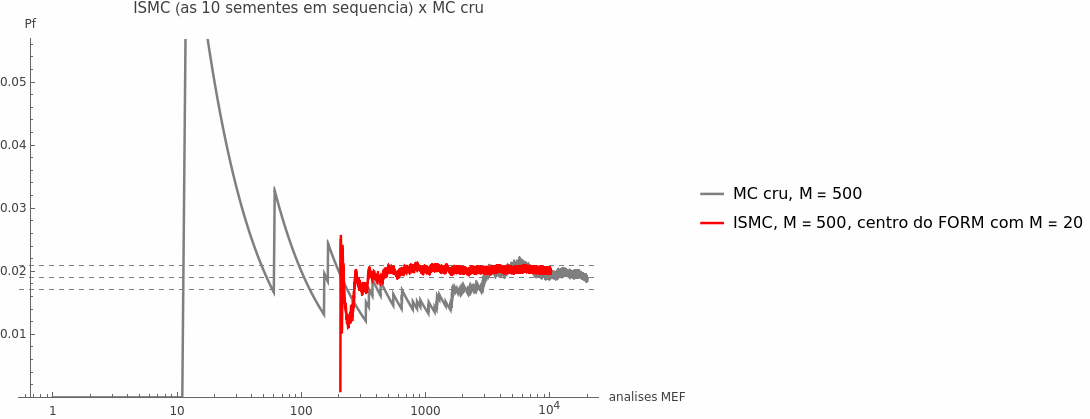
\includegraphics[width=0.75\textwidth]{figs/gConvCampo.png}
\caption{ISMC no campo de 500 modos com o centro do FORM de 20 (10 sementes em sequência) contra o MC direto.}
\end{figure}

\section{FORM com 5 termos e ISMC com 200: as figuras}
FORM com $M = 5$: $\beta = 2{,}277$ em 55 análises; ISMC com o campo de 200: $P_f = 2{,}02\,\%$ (CoV 7,3\,\%) contra
2,14\,\% do MC de 20\,000 ($z = -0{,}69$); ESS$_F$ = 159, maior parcela 3,8\,\%.
\begin{figure}[H]\centering
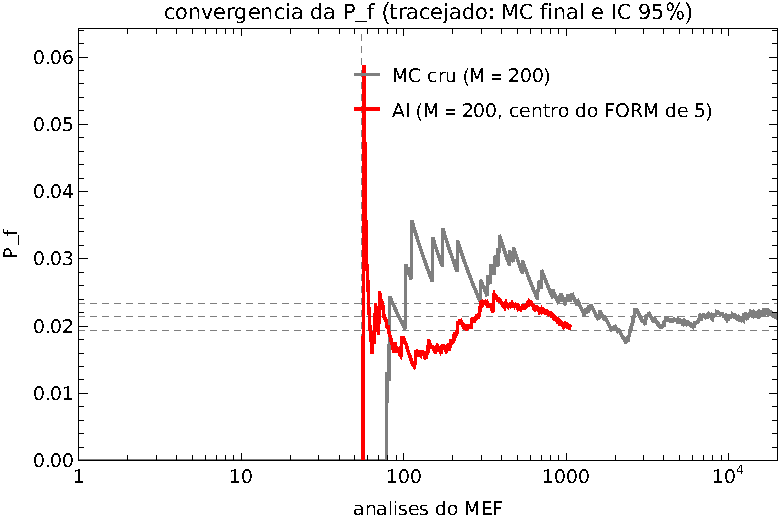
\includegraphics[width=0.48\textwidth]{figs/pf_convergencia.pdf}\hfill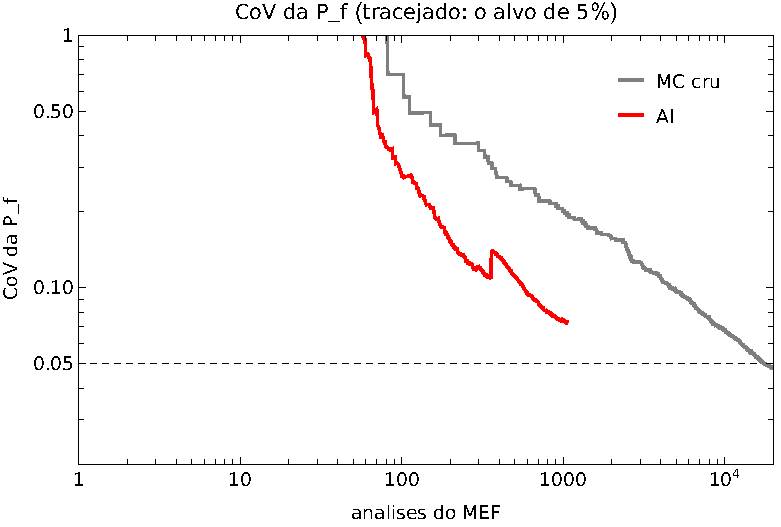
\includegraphics[width=0.48\textwidth]{figs/cov_convergencia.pdf}
\caption{Convergência da $P_f$ e do CoV: a ISMC começa depois das 55 análises do FORM.}
\end{figure}
\begin{figure}[H]\centering
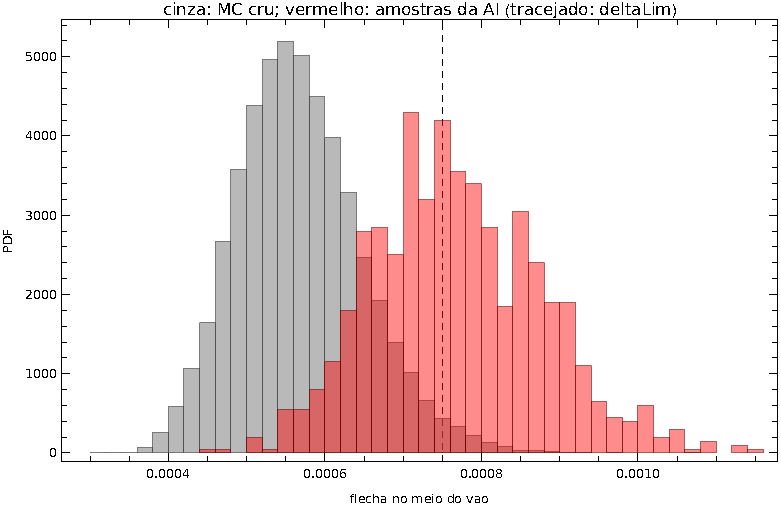
\includegraphics[width=0.48\textwidth]{figs/histograma_flechas.pdf}\hfill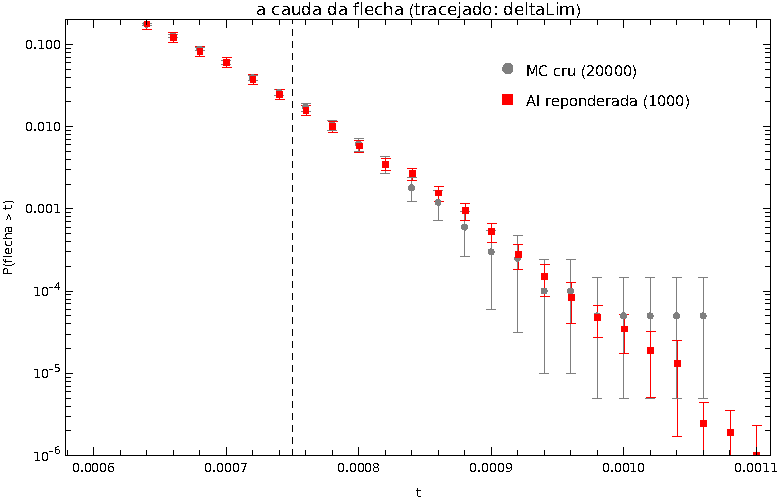
\includegraphics[width=0.48\textwidth]{figs/cauda.pdf}
\caption{As flechas do MC e as amostras da ISMC; a cauda $P(\delta > t)$ pela ISMC reponderada (1000) e pelo MC (20\,000).}
\end{figure}
\begin{figure}[H]\centering
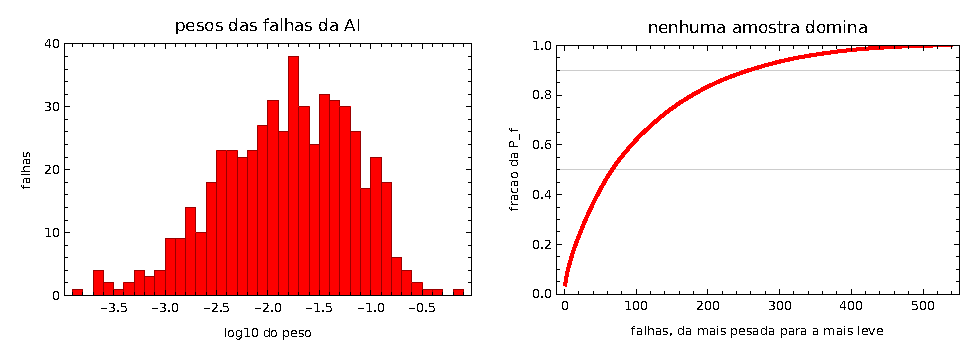
\includegraphics[width=0.62\textwidth]{figs/pesos.pdf}\hfill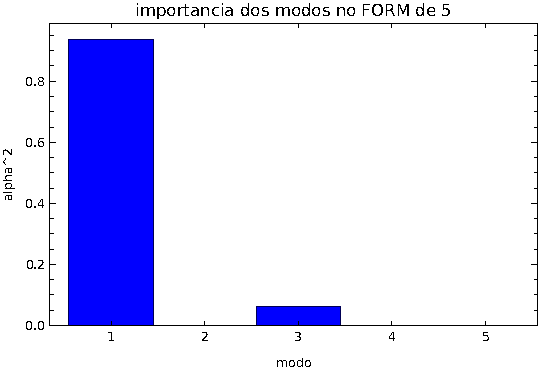
\includegraphics[width=0.36\textwidth]{figs/alpha2.pdf}
\caption{Os pesos das falhas da ISMC (nenhuma amostra domina) e os $\alpha^2$ do FORM de 5.}
\end{figure}
\begin{figure}[H]\centering
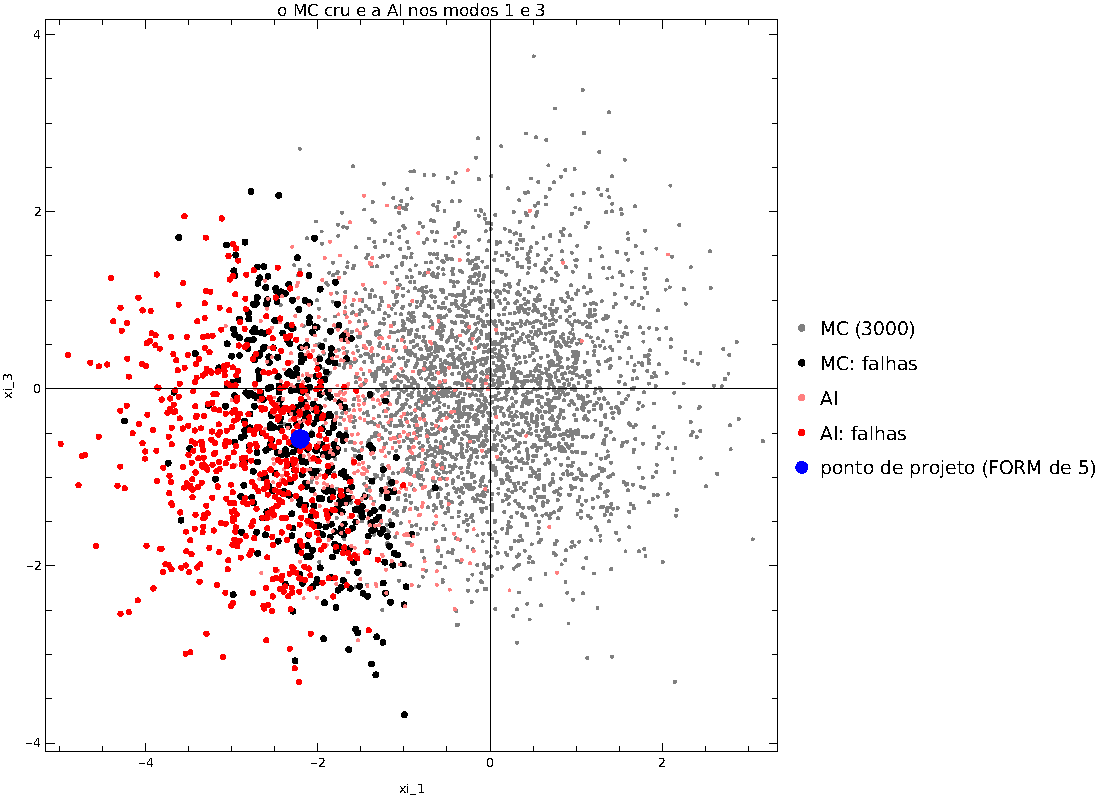
\includegraphics[width=0.55\textwidth]{figs/xi_modos_1_3.pdf}\hfill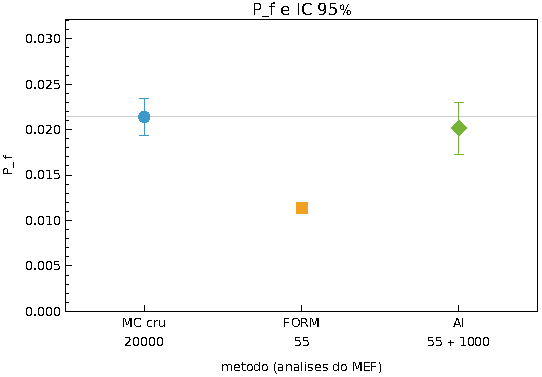
\includegraphics[width=0.40\textwidth]{figs/pf_metodos.pdf}
\caption{As amostras nos modos 1 e 3 e a $P_f$ de cada método.}
\end{figure}

\section{O ponto ótimo do M do FORM}
Referência: MC direto de 50\,000 com $M = 200$, $P_f = 2{,}098\,\%$ (CoV 3,05\,\%; 18\,666 análises para CoV de 5\,\%).
\begin{table}[H]\centering\small
\resizebox{\ifdim\width>\textwidth\textwidth\else\width\fi}{!}{%
\begin{tabular}{rrrrrrrrr}
\toprule
$M$ & $P_f$ FORM & erro & análises FORM & $P_f$ ISMC (1000) & erro & $z$ & total p/ CoV 5\,\% & ganho \\
\midrule
2 & 0,95\,\% & $-55\,\%$ & 25 & 2,16\,\% & +3,0\,\% & 0,40 & 3566 & 5,2$\times$ \\
3 & 1,14\,\% & $-46\,\%$ & 35 & 2,25\,\% & +7,3\,\% & 0,96 & 2187 & 8,5$\times$ \\
5 & 1,14\,\% & $-46\,\%$ & 55 & 2,25\,\% & +7,3\,\% & 0,96 & 2208 & 8,5$\times$ \\
8 & 1,58\,\% & $-25\,\%$ & 85 & 2,29\,\% & +9,1\,\% & 1,42 & \textbf{1198} & \textbf{15,6}$\times$ \\
10 & 1,58\,\% & $-25\,\%$ & 105 & 2,29\,\% & +9,1\,\% & 1,42 & 1218 & 15,3$\times$ \\
15 & 1,58\,\% & $-25\,\%$ & 155 & 2,29\,\% & +9,1\,\% & 1,42 & 1267 & 14,7$\times$ \\
20 & 1,66\,\% & $-21\,\%$ & 205 & 2,20\,\% & +4,9\,\% & 0,83 & 1224 & 15,2$\times$ \\
30 & 1,66\,\% & $-21\,\%$ & 305 & 2,20\,\% & +4,8\,\% & 0,83 & 1324 & 14,1$\times$ \\
40 & 1,66\,\% & $-21\,\%$ & 405 & 2,22\,\% & +5,7\,\% & 0,96 & 1419 & 13,2$\times$ \\
60 & 1,67\,\% & $-20\,\%$ & 605 & 2,22\,\% & +5,8\,\% & 0,99 & 1607 & 11,6$\times$ \\
100 & 1,70\,\% & $-19\,\%$ & 1005 & 2,20\,\% & +5,0\,\% & 0,86 & 1959 & 9,5$\times$ \\
200 & 1,71\,\% & $-19\,\%$ & 2005 & 2,21\,\% & +5,2\,\% & 0,90 & 2951 & 6,3$\times$ \\
\bottomrule
\end{tabular}}
\caption{ISMC sempre com o campo de 200 e o centro do FORM de $M$ termos. O total usa o CoV verdadeiro. As ISMC usam a
mesma semente (números aleatórios comuns), então os seus erros andam juntos e não são conferências independentes.}
\end{table}
\begin{figure}[H]\centering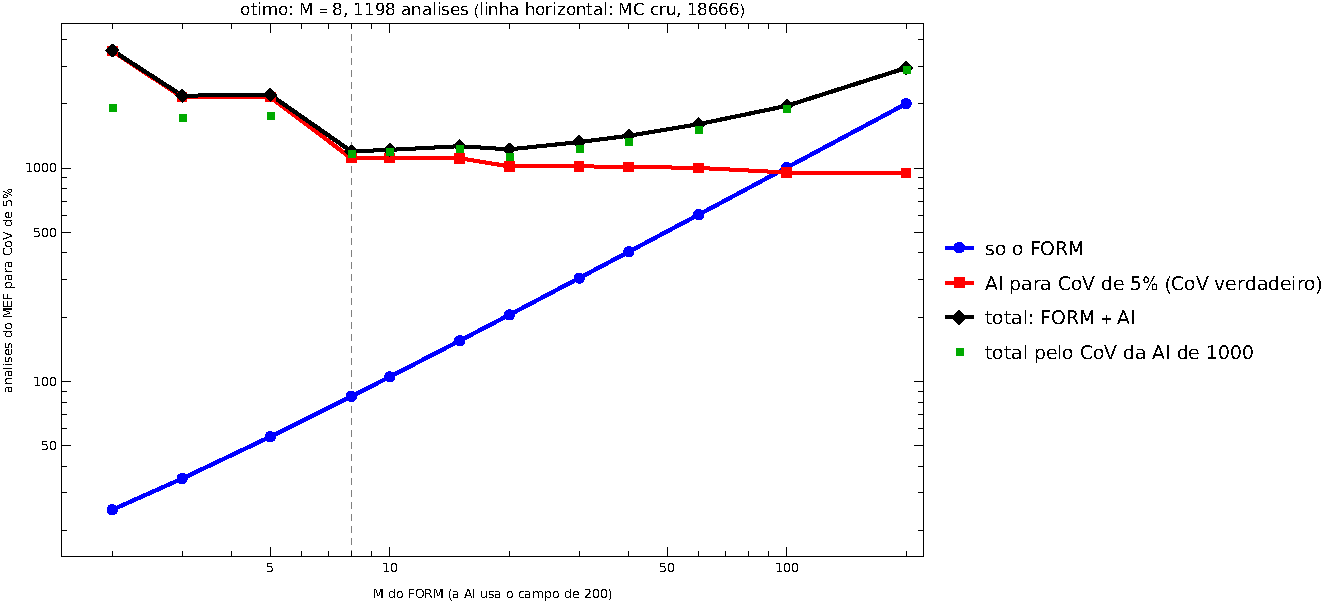
\includegraphics[width=0.8\textwidth]{figs/ponto_otimo.pdf}
\caption{O custo do FORM sobe em linha reta com $M$; o da ISMC cai em degraus quando entram os modos importantes (3, 8 e
16). O ótimo é um patamar de $M = 8$ a 20.}
\end{figure}

\section{SORM}
Todas as curvaturas são negativas (a região de falha é maior que o semiespaço do FORM); com $M = 200$ as maiores são
$-0{,}055$, $-0{,}031$, $-0{,}024$ e $-0{,}017$, soma $-0{,}14$.
\begin{table}[H]\centering\small
\resizebox{\ifdim\width>\textwidth\textwidth\else\width\fi}{!}{%
\begin{tabular}{rrrrrrrr}
\toprule
$M$ & $P_f$ FORM & erro & SORM Breitung & erro & SORM H-R & erro & análises FORM + hessiano \\
\midrule
2 & 0,947\,\% & $-55\,\%$ & 1,003\,\% & $-52\,\%$ & 1,011\,\% & $-52\,\%$ & 25 + 7 \\
5 & 1,139\,\% & $-46\,\%$ & 1,297\,\% & $-38\,\%$ & 1,324\,\% & $-37\,\%$ & 55 + 31 \\
8 & 1,584\,\% & $-25\,\%$ & 1,800\,\% & $-14\,\%$ & 1,840\,\% & $-12\,\%$ & 85 + 73 \\
10 & 1,584\,\% & $-25\,\%$ & 1,830\,\% & $-13\,\%$ & 1,877\,\% & $-11\,\%$ & 105 + 111 \\
20 & 1,657\,\% & $-21\,\%$ & 1,938\,\% & $-8\,\%$ & 1,992\,\% & $-5\,\%$ & 205 + 421 \\
40 & 1,660\,\% & $-21\,\%$ & 1,969\,\% & $-6\,\%$ & 2,029\,\% & $-3\,\%$ & 405 + 1641 \\
100 & 1,702\,\% & $-19\,\%$ & 2,006\,\% & $-4\,\%$ & 2,066\,\% & $-1{,}5\,\%$ & 1005 + 10\,101 \\
200 & 1,707\,\% & $-19\,\%$ & 2,002\,\% & $-5\,\%$ & 2,060\,\% & $-1{,}8\,\%$ & 2005 + 40\,201 \\
\bottomrule
\end{tabular}}
\caption{FORM e SORM contra o MC direto de 50\,000 (IC 95\,\%: $\pm 6\,\%$). Com $M$ pequeno o erro é de truncamento:
o SORM com 5 termos (1,32\,\%) dá a $P_f$ do MC com 5 termos (1,33\,\%).}
\end{table}
\begin{figure}[H]\centering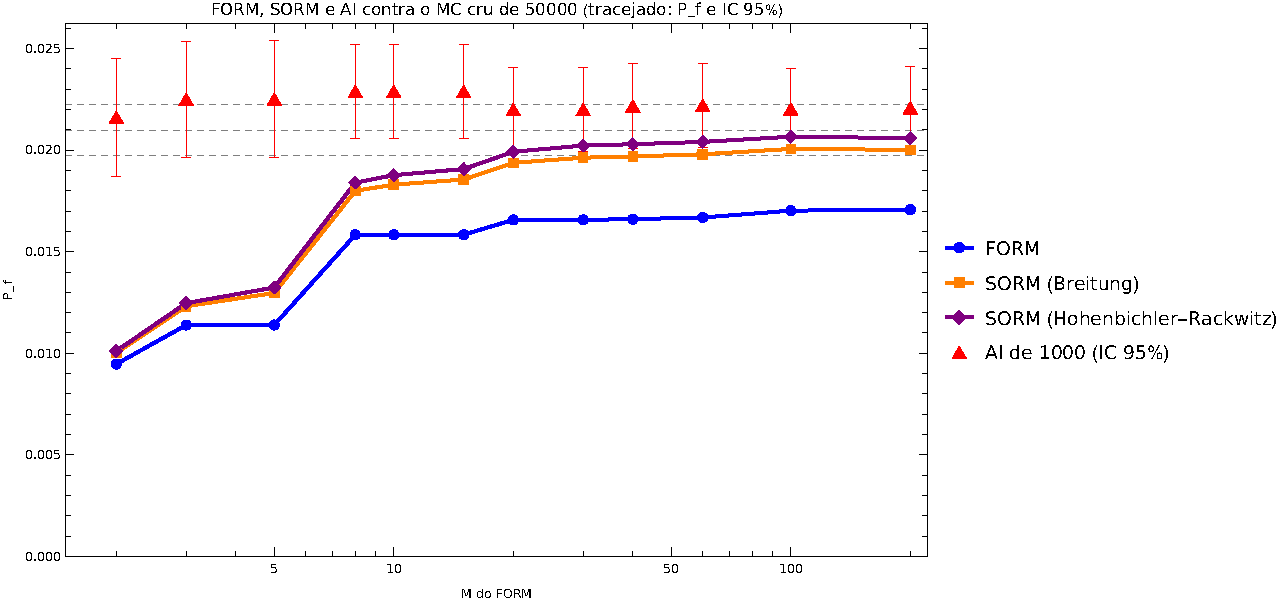
\includegraphics[width=0.8\textwidth]{figs/form_sorm_ai.pdf}
\caption{FORM, SORM e ISMC contra o MC direto de 50\,000.}
\end{figure}

\section{O SORM como função de amostragem: a verificação}
\begin{table}[H]\centering\small
\resizebox{\ifdim\width>\textwidth\textwidth\else\width\fi}{!}{%
\begin{tabular}{lrrrrrr}
\toprule
densidade ($M = 20$, 10 $\times$ 1000) & $P_f$ (média) & CoV entre sementes & CoV estimado & erro & $z$ & $N$ p/ CoV 5\,\% \\
\midrule
FORM: $N(\bm\xi^*, I)$ & 1,989\,\% & 5,01\,\% & 5,15\,\% & $-5{,}2\,\%$ & $-1{,}53$ & 1004 \\
SORM Breitung: $N(\bm\xi^*, \Sigma)$ & 1,996\,\% & 4,99\,\% & 5,08\,\% & $-4{,}8\,\%$ & $-1{,}42$ & 996 \\
SORM H-R: $N(\bm\xi^*, \Sigma)$ & 1,997\,\% & 4,87\,\% & 5,08\,\% & $-4{,}8\,\%$ & $-1{,}42$ & 949 \\
\bottomrule
\end{tabular}}
\caption{As mesmas sementes nas três densidades. A diferença SORM $-$ FORM semente a semente é $+0{,}38 \pm 0{,}34\,\%$
(Breitung) e $+0{,}43 \pm 0{,}44\,\%$ (H-R): nenhuma.}
\end{table}
\begin{table}[H]\centering\small
\resizebox{\ifdim\width>\textwidth\textwidth\else\width\fi}{!}{%
\begin{tabular}{rrrrrrr}
\toprule
$M$ & $N$ FORM & $N$ SORM B & SORM/FORM & hessiano & total ISMC-FORM & total ISMC-SORM \\
\midrule
5 & 2153 & 2129 & 0,989 & 31 & 2208 & 2215 \\
8 & 1113 & 1097 & 0,986 & 73 & \textbf{1198} & 1255 \\
20 & 1019 & 997 & 0,978 & 421 & 1224 & 1623 \\
60 & 1002 & 980 & 0,978 & 3661 & 1607 & 5246 \\
200 & 946 & 923 & 0,975 & 40\,201 & 2951 & 43\,129 \\
\bottomrule
\end{tabular}}
\caption{Amostras para CoV de 5\,\% pelo CoV verdadeiro de cada densidade.}
\end{table}
\begin{figure}[H]\centering
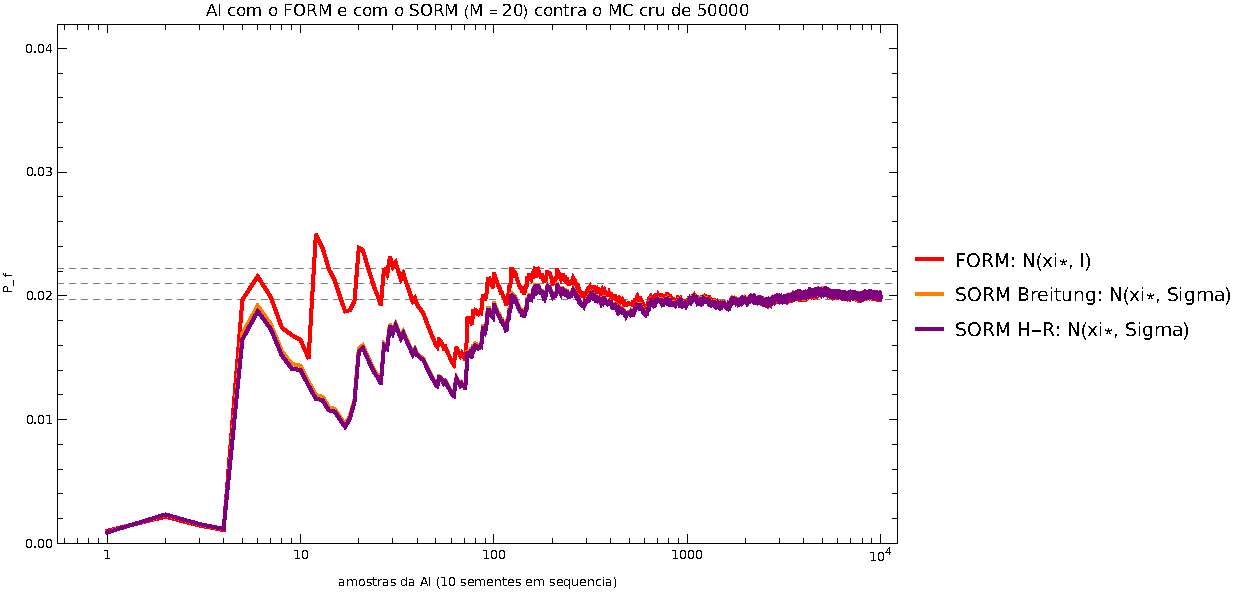
\includegraphics[width=0.48\textwidth]{figs/verif_sorm_form_pf.pdf}\hfill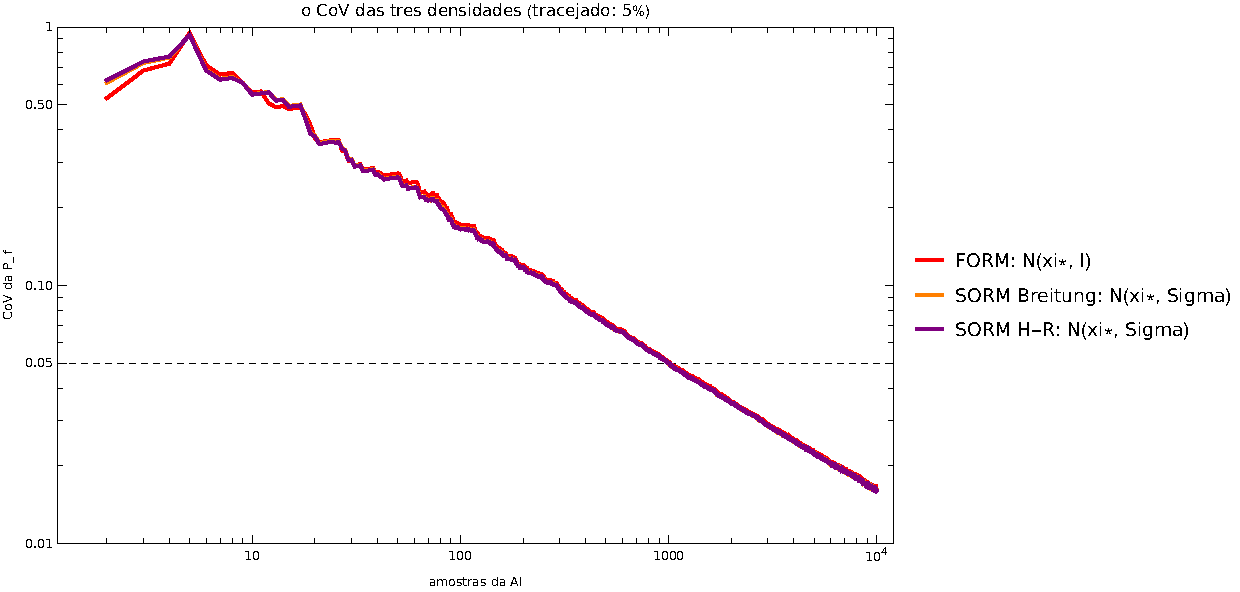
\includegraphics[width=0.48\textwidth]{figs/verif_sorm_form_cov.pdf}\\
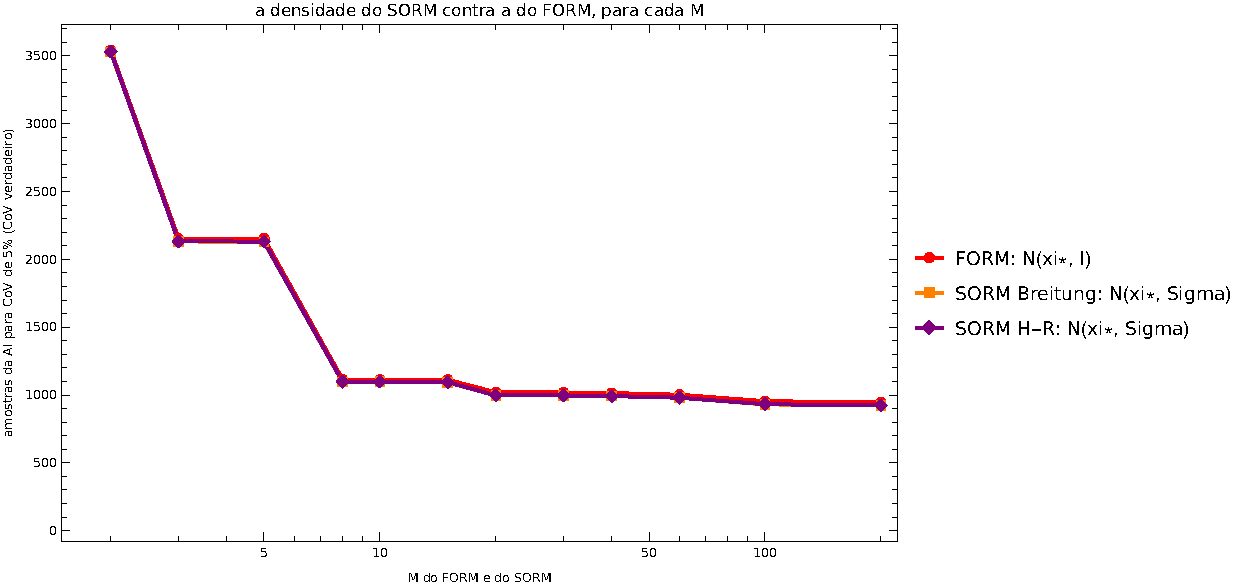
\includegraphics[width=0.6\textwidth]{figs/verif_sorm_form_M.pdf}
\caption{A convergência das três densidades (10 sementes em sequência) e o $N$ para CoV de 5\,\% com $M$.}
\end{figure}

\section{Conclusões}
\begin{enumerate}
  \item A ISMC não tem viés com nenhum centro testado (FORM de 2 a 200 termos, fórmulas TG e EB, SORM): o centro só muda
    a variância. O CoV estimado bate com o verdadeiro e com a dispersão entre sementes.
  \item O FORM sozinho erra a $P_f$ em $-19$ a $-55\,\%$; o ponto de projeto, porém, é uma boa função de amostragem.
  \item O FORM precisa só dos modos com $\alpha^2$ relevante (1, 3, 8 e 16 aqui): o ótimo é $M = 8$ a 20, $\approx 1200$
    análises para CoV de 5\,\% (15$\times$ menos que o MC). Mais termos só encarecem o gradiente numérico.
  \item Um modelo barato (a fórmula de viga TG) dá o centro sem custo de MEF: 19$\times$ com o campo de 200.
  \item O SORM (H-R) corrige a $P_f$ do FORM para $-5\,\%$ com $M = 20$ (626 análises), mas não informa o próprio erro.
    Como função de amostragem, reduz as amostras em só 1 a 2,5\,\% (curvaturas pequenas) e o hessiano custa mais do que
    economiza.
  \item Para o talude (etapa 3b): FORM com poucos termos (20) e gradiente numérico ou modal para o centro, e a ISMC no
    campo completo.
\end{enumerate}
\end{document}
